\documentclass{article}
\usepackage[UTF8]{ctex}
\setmainfont{Calibri Light}
\usepackage{setspace}
\renewcommand{\baselinestretch}{1.2}
\usepackage{amsmath}
\usepackage{amssymb}
\usepackage{ntheorem}
\usepackage{graphicx}
\usepackage{bbm}
\usepackage{hyperref}
\hypersetup{
	colorlinks=true,
	linkcolor=blue,
	filecolor=cyan,      
	urlcolor=red,
	citecolor=green,
}
\newtheorem{theorem}{Theorem}
\newtheorem{corollary}{Corollary}
\newtheorem{lemma}{Lemma}
\newtheorem*{proof}{Proof}
\setlength{\parindent}{2em}
\author{Siheng Zhang\\zhangsiheng@cvte.com}
\title{Chapter \textbf{\textit{4}}\ \ \ \ 线性模型}
\date{\today}
\usepackage[a4paper,left=18mm,right=18mm,top=25mm,bottom=25mm]{geometry} 

\begin{document}
\maketitle  

This part corresponds to \textbf{Chapter 1,3,4 of PRML, Chapter of UML}, and mainly answers the following questions:

\begin{itemize}
\item 
\end{itemize}

\tableofcontents
\newpage

\section{线性分类器}

	上一章的结尾,我们引出了二分类问题的线性分类器,形如
	
	\begin{equation}
	y=h(\mathbf{x})=\mathbf{w}^\top \mathbf{x} + w_0 = \sum_{j=1}^d w_j x_j + w_0
	\label{eq:linear}
	\end{equation}
其中$\mathbf{w}$代表权重向量,$w_0$代表偏置。样本被分类为$C_1$当且仅当$h(\mathbf{x})\geq 0$,否则分类为$C_2$。

	考虑两个在决策面上的点$\mathbf{x}_1,\mathbf{x}_2$,即$\mathbf{w}^\top (\mathbf{x}_1 - \mathbf{x}_2) = 0$,因此$\mathbf{w}$正交于决策面。此外,原点到决策面的距离为$\mathbf{w}^\top \mathbf{x} / \|\mathbf{w}\|=-w_0/\|\mathbf{w}\|$。
	
	\vspace{2mm}
	\begin{scriptsize}
	\begin{spacing}{1.2}
	{\sffamily
	\noindent\textit{\underline{remark1.} 通常引入增广维度$x_0 = 1$,并定义$\tilde{\mathbf{w}} = (w_0, \mathbf{w})$与$\tilde{\mathbf{x}} = (x_0, \mathbf{x})$,则$h(\mathbf{x}) = \tilde{\mathbf{w}}^\top \tilde{\mathbf{x}}$。在不引起误会的情况下,下文隐去波浪号。}
	
	\noindent\textit{\underline{remark2: 多类别情况。}  \textbf{一对多} 对每个类别判断是与否,因此需要$K$个分类器;  \textbf{一对一} 为每对类别引入一个分类器,因此需要$K(K-1)/2$个分类器(但是会出现“真空”地带)。}}
	\end{spacing}
	\end{scriptsize}
	\vspace{-2mm}
	
	\subsection{线性分类器的VC维}
	
	带偏置的线性分类的VC维为:$VCdim(HS_d)=d+1$.  

	\vspace{2mm}
	\begin{scriptsize}
	\begin{spacing}{1.2}
	{\sffamily
	\noindent\textit{\underline{remark3: proof.}} Firstly, we should show that any set of $d$ points in $\mathcal{R}^d$ can be shattered by half-space. 
	
	Secondly, we should show there exists a point set of $d+1$ points in $\mathcal{R}^{d}$ that cannot be shattered by half-space. Denote the points as $\mathbf{x}_1, \mathbf{x}_2, \cdots, \mathbf{x}_{d+1}$. There must be some $a_i, i=1,2,\cdots,d+1$ (not all of them are zero) which satisfy that $\sum_{i=1}^{d+1} a_i \mathbf{x}_i = \mathbf{0}$. Split the $a_i$ into two sets $I={i,a_i>0}$ and $J={i,a_i<0}$, then we have 
	\begin{equation*}
	\sum_{i\in I} a_i \mathbf{x}_i = \sum_{i \in J} |a_i| \mathbf{x}_i
	\end{equation*}
If the VC dimension is $d+1$, then there must be some $\mathbf{w}$ such that $\mathbf{w}^\top \mathbf{x}_i > 0, \forall i \in I$ and $\mathbf{w}^\top \mathbf{x}_i < 0, \forall i \in J$. It follows that
	
	\begin{equation*}
	0 < \sum_{i \in I} a_i \mathbf{w}^\top \mathbf{x}_i = \mathbf{w}^\top  \sum_{i \in I} a_i \mathbf{x}_i = \mathbf{w}^\top  \sum_{i \in J} |a_i| \mathbf{x}_i =  \sum_{i \in J} |a_i| \mathbf{w}^\top \mathbf{x}_i  < 0
	\end{equation*}
which leads to a contradiction.}
	\end{spacing}
	\end{scriptsize}
	
	It follows that we can learn half-space using the ERM paradigm with a sample size of $\Omega(\frac{d+\log(1/\delta)}{\epsilon})$. Before discussing the implementation, we would like to show that the bound of sample size is too loose, and hence loss its guiding meaning in practice.  Suppose that we would like to be 'very sure' to the learned hypothesis, namely $\epsilon\rightarrow 0$ and $\delta\rightarrow 1$, then the sample size tends to be infinity. In agnostic case, since we cannot learn  a perfect half space, naturally  more training data is better, and the estimation of samples size is trivial. In realizable case, since 
	
	In the realizable (namely, separable) case, we can implement ERM paradigm as a linear programming problem. The normal form of a linear programming problem is:
	
	\begin{equation*}
	\begin{split}
	&\min_\mathbf{w} \mathbf{u}^\top \mathbf{w} \\
	s.t. & \mathbf{Aw} \geq \mathbf{v}
	\end{split}
	\end{equation*}
	
Besides, we can also use a Perceptron algorithm, which is left in the next chapter.
	
	However, in the agnostic (namely, non-separable) case, the implementation is computational hard. And the most popular solution is to use \textit{surrogate loss} functions but not the 0-1 loss in realizable case. ......
	
	\subsection{费舍(Fisher)线性判别}
	
	线性分类从另一个角度可以看成是\textit{降维},即从$\mathcal{R}^d$空间向$\mathcal{R}$的变换。通过调整权重向量,我们可以找到一个最大化类间距离的变换。考虑二分类问题,其中类$C_1$有$N_1$个样本点,类$C_2$有$N_2$个样本点。则两个类的均值向量为:

	\begin{equation*}
	\mathbf{m}_i = \frac{1}{N_i} \sum_{\mathbf{x} \in C_i} \mathbf{x}, \ \ \ \ i=1,2
	\end{equation*}
	
	如何评价降维后的类间距离?最直接的想法就是使用降维后的类均值的差,即
	\begin{equation*}
	\max_\mathbf{w} m_2- m_1=\mathbf{w}^\top (\mathbf{m}_2-\mathbf{m}_1)
	\end{equation*}
其中$m_k=\mathbf{w}^\top \mathbf{m}_k$。

	注意到,如不限制$\mathbf{w}$的模,该值可以无限大。因此需要限制$\|\mathbf{w}\|_2=1$。使用拉格朗日乘子法,优化目标转化为$\mathbf{w}^\top (\mathbf{m}_2-\mathbf{m}_1) + \lambda (1-\|\mathbf{w}\|_2)$,从而推出$\mathbf{w}\propto \mathbf{m}_2-\mathbf{m}_1$。
	
	但这种方法是有缺陷的,即使数据集线性可分,这种投影也会将一些点(如图)误分类。事实上,除了最大化类间距离,投影还应该最小化类内方差。记方差为$s_k^2=\sum_{\mathbf{x}_n\in C_k} (\mathbf{w}^\top\mathbf{x}_n-m_k)^2$,则优化目标为:
	
	\begin{equation}
	\max_\mathbf{w} J(\mathbf{w}) = \frac{(m_2-m_1)^2}{s_1^2+s_2^2} 
	= \frac{\mathbf{w}^\top \left[ (\mathbf{m}_2-\mathbf{m}_1)(\mathbf{m}_2-\mathbf{m}_1)^\top \right] \mathbf{w}}{\mathbf{w}^\top \left[ \sum_{i=1}^2 \sum_{\mathbf{x}_n\in C_i}(\mathbf{x}_n-\mathbf{m}_1)(\mathbf{x}_n-\mathbf{m}_1)^\top\right] \mathbf{w}}
	\overset{def}{=} \frac{\mathbf{w}^\top \mathbf{S}_B \mathbf{w}}{\mathbf{w}^\top \mathbf{S}_W \mathbf{w}}
	\end{equation}
其最优解(其解留为练习)为:
	\begin{equation*}
	\mathbf{w}\propto \mathbf{S}_W^{-1} (\mathbf{m}_2-\mathbf{m}_1)
	\end{equation*}
	
	\begin{scriptsize}
	\begin{spacing}{1.2}
	{\sffamily \textit{\underline{remark4: Fisher's linear discriminant for the case of multi-class.}}}
	\end{spacing}
	\end{scriptsize}
	
	\subsection{最小二乘法用于分类问题}
	
	\subsection{概率视角}
	
	\subsubsection{逻辑斯特(Logistics)回归}
	
	\subsubsection{迭代重加权最小二乘法(Iterative re-weighted least squares,IRLS)}

\section{线性回归}

	线性回归模型与分类模型形式相同,除了标签$y$是连续的而非离散的,且优化目标为误差平方和(sum-of-square,SSE):

	\begin{equation}
	\min_\mathbf{w} L_S(h) =\sum_{i=1}^m  l(h(\mathbf{x}_i)) = \sum_{i=1}^m (h(\mathbf{x}_i) - y_i)^2 = \sum_{i=1}^m (\mathbf{w}^\top\mathbf{x}_i - y_i)^2 
	\end{equation}

	假设拟合误差$\epsilon_i = y_i-\mathbf{wx}_i$是高斯噪声,即$\epsilon_i \sim\mathcal{N}(0,\beta)$,则训练集的对数似然为:
	
	\begin{equation}
	\log \mathcal{L} = -\frac{m}{2} \log 2\pi\beta - \sum_{i=1}^m \frac{(y_i-\mathbf{w}^\top\mathbf{x}_i)^2}{2\beta}
	\end{equation}

显然,极大似然的结果等价于线性回归。

	\vspace{2mm}
	\begin{scriptsize}
	\begin{spacing}{1.2}
	{\sffamily
	\noindent \textit{\underline{注5.} Since linear regression is not a binary prediction task, we cannot analyse its sample complexity using the VC-dimension. One possible analysis of the sample complexity of linear regression is by relying on the "discretization trick". However, to apply the sample complexity bounds from Chapter 2 we also need that the loss function will be bounded.}}
	\end{spacing}
	\end{scriptsize}
	\vspace{-2mm}
	
	\subsection{广义线性回归}
	
	The model is just a linear function of the input variables, and this imposes significant limitations on it. Therefore, extended model considers \textbf{linear} combination of fixed \textbf{non-linear} functions of the input variables, of the form
	
	\begin{equation}
	h(\mathbf{x}) = w_0 + \sum_{j=1}^d w_j \phi_j(x)
	\end{equation}
where $\phi_j(x)$ are known as \textit{basis functions}. Again, denote $\phi_0(\mathbf{x})=1$ so that $h(\mathbf{x}) = \tilde{\mathbf{w}}^\top \phi(\mathbf{x})$. For Simplification, we also neglect the `tilde' symbol from now on.

	Now, consider the closed-form solution for The gradient of the log likelihood. The gradient of the SSE loss takes the form
	
	\begin{equation*}
	\nabla L_S(h) = \sum_{i=1}^m \left\{ y_i - \mathbf{w}^\top \mathbf{\phi} (\mathbf{x}_i)) \right\} \mathbf{\phi}^\top (\mathbf{x}_i)
	\end{equation*}
Setting it to zero gives 

	\begin{equation}
	\label{eqn:mp_solved}
	\mathbf{w} = \Phi^\dag \mathbf{y} = (\Phi^\top \Phi)^{-1} \Phi^\top \mathbf{y}
	\end{equation}
Here $\Phi$ is an $n*d$ matrix, whose elements are given by $\Phi_{nj} = \phi_j(\mathbf{x}_n)$. And $\Phi^\dag$ is \textit{Moore-Penrose pseudo-inverse}.

	\vspace{2mm}
	\begin{scriptsize}
	\begin{spacing}{1.2}
	{\sffamily 
	\textit{\underline{remark6: multiple-outputs.}} A more general case is multiple outputs, i.e., $\mathbf{y}_i \in \mathcal{R}^k, k>1$. However, the solution to multiple-outputs regression problem decouples between the different target variables so we do not discuss it here.
	
	\textit{\underline{remark7: on-line learning.}} Batch techniques involve processing the entire training set in one go, can be computationally costly for large data sets. For linear regression, stochastic gradient descent algorithm updates parameter using
	
	\begin{equation*}
	\mathbf{w}^{t+1}=\mathbf{w}^{t} - lr*\nabla L_{(\mathbf{x}_t,y_t)}(h) = \mathbf{w}^{t} + lr* (y_i - (\mathbf{w}^t)^\top \mathbf{\phi} (\mathbf{x}_t)) \mathbf{\phi} (\mathbf{x}_t)
	\end{equation*}
in which $lr$ is the learning rate.

	\textit{\underline{remark8: Basis function examples.}} 1. \textbf{Polynomial basis}, 2. \textbf{Radical basis}, 3. \textbf{Fourier basis}.
	}
	\end{spacing}
	\end{scriptsize}
	\vspace{-2mm}
	
	\subsection{正则化与贝叶斯线性回归}
	
	In closed-form solution (Eq. \ref{eqn:mp_solved}), if $n\leq d$, the SSE loss can achieve zero. It means that the model capacity is enough to 'memorize' all training examples. But it may suffer from \textbf{over-fitting}.
	
	Consider the expected loss with squared error,
	\begin{equation}
	\begin{split}
	\mathbb{E}(l) &= \int \int l(h(\mathbf{x})) p(\mathbf{x}, y) \text{d} \mathbf{x} \text{d}y \\
	&= \int \int (h(\mathbf{x})-y)^2 p(\mathbf{x}, y) \text{d} \mathbf{x} \text{d}y
	\ \ \ \ \footnotesize{\text{Note that, setting its derivatives to zero leads to $h(\mathbf{x}) = \int yp(\mathbf{x}, y) \text{d} y /p(\mathbf{x}) = \mathbb{E}(y|\mathbf{x})$}}\\
	&= \int \int \left\{ h(\mathbf{x}) - \mathbb{E} (y|\mathbf{x}) + \mathbb{E} (y|\mathbf{x}) - y \right\}^2 p(\mathbf{x}, y) \text{d} \mathbf{x} \text{d}y \\
	&= \int \int \left\{ \left[ h(\mathbf{x}) - \mathbb{E} (y|\mathbf{x}) \right]^2 + \left[\mathbb{E} (y|\mathbf{x}) - y \right]^2 + 2 \left[ h(\mathbf{x}) - \mathbb{E} (y|\mathbf{x}) \right] \left[\mathbb{E} (y|\mathbf{x}) - y \right]  \right\} p(\mathbf{x}, y) \text{d} \mathbf{x} \text{d}y \\
	&= \int \left\{ h(\mathbf{x}) - \mathbb{E} (y|\mathbf{x}) \right\}^2 p(\mathbf{x}) \text{d} \mathbf{x} + \int \int \left\{\mathbb{E} (y|\mathbf{x}) - y \right\}^2 p(\mathbf{x}, y) \text{d} \mathbf{x} \text{d} y
	\end{split}
	\end{equation}
	
	The second term, which is independent of $h(\mathbf{x})$, arises from the intrinsic noise on the data and represents the minimum achievable value of the expected loss. The first term depends on our choice for the function $h(\mathbf{x})$. Because it is non-negative, its optimal value is zero. If we had an unlimited supply of data (and unlimited computational resources), we could in principle find the regression function $h(\mathbf{x})$ to any desired degree of accuracy.
	
	Consider the integrand of the first term. For a particular data set $\mathcal{D}$, the expectation is not depend on the data set, but the function $h(\cdot)$ does. So it takes the form
	
	\begin{equation*}
	\begin{split}
	  & \left\{ h(\mathbf{x};\mathcal{D})- \mathbb{E}(y|\mathbf{x}) \right\}^2 \\
	= & \left\{ h(\mathbf{x};\mathcal{D})- \mathbb{E}_\mathcal{D}(h(\mathbf{x};\mathcal{D})) + \mathbb{E}_\mathcal{D}(h(\mathbf{x};\mathcal{D})) - \mathbb{E}(y|\mathbf{x}) \right\}^2 \\
	= & \left\{ h(\mathbf{x};\mathcal{D})- \mathbb{E}_\mathcal{D}(h(\mathbf{x};\mathcal{D}))\right\}^2 + \left\{ \mathbb{E}_\mathcal{D}(h(\mathbf{x};\mathcal{D})) - \mathbb{E}(y|\mathbf{x}) \right\}^2 + 2 \left\{ h(\mathbf{x};\mathcal{D})- \mathbb{E}_\mathcal{D}(h(\mathbf{x};\mathcal{D}))\right\} \left\{ \mathbb{E}_\mathcal{D}(h(\mathbf{x};\mathcal{D})) - \mathbb{E}(y|\mathbf{x}) \right\} \\
	\end{split}
	\end{equation*}
Now take expectation of it with respect to $\mathcal{D}$, the third term will vanish, giving 

	\begin{equation}
	\begin{split}
	\mathbb{E}_\mathcal{D} \left[ \left\{ h(\mathbf{x};\mathcal{D})- \mathbb{E}(y|\mathbf{x}) \right\}^2 \right]
	&= \mathbb{E}_\mathcal{D} \left[ \left\{ \mathbb{E}_\mathcal{D}(h(\mathbf{x};\mathcal{D})) - \mathbb{E}(y|\mathbf{x}) \right\}^2 \right] + \mathbb{E}_\mathcal{D} \left[ \left\{ h(\mathbf{x};\mathcal{D})- \mathbb{E}_\mathcal{D}(h(\mathbf{x};\mathcal{D}))\right\}^2 \right] \\
	&= \underbrace{\left\{ \mathbb{E}_\mathcal{D}(h(\mathbf{x};\mathcal{D})) - \mathbb{E}(y|\mathbf{x}) \right\}^2}_{\text{bias}^2} + \underbrace{\mathbb{E}_\mathcal{D} \left[ \left\{ h(\mathbf{x};\mathcal{D})- \mathbb{E}_\mathcal{D}(h(\mathbf{x};\mathcal{D}))\right\}^2 \right]}_{\text{variance}}
	\end{split}
	\end{equation}
The first term, called the squared bias, represents the extent to which the average prediction over all data sets differs from the desired regression function. The second term, called the variance, measures the extent to which the solutions for individual data sets vary around their average, and hence this measures the extent to which the regressor is sensitive to the particular choice of data set.

	As discussed before, there is a trade-off between bias and variance, with very flexible models having low bias and high variance, and relatively rigid models having high bias and low variance. Bayesian linear regression set a prior assumption of $\mathbf{w}$, and view the learning procedure to maximizing its posterior. Two of the most popular case is discussed below. 

\subsubsection{岭回归(Ridge regression)}

	岭回归通过惩罚权重的$l_2$范数来解决过拟合问题,
	
	\begin{equation*}
	\min_\mathbf{w} \sum_{i=1}^m (\mathbf{w\phi}_i(\mathbf{x}) - y_i)^2 + \lambda\|\mathbf{w}\|^2_2
	\end{equation*}

	如果假设权重的先验分布为高斯分布,$\mathbf{w}\sim\mathcal{N}(0,\alpha^{-1}\mathbf{I})$,则其后验为:
	
	\begin{equation}
	p(\mathbf{w}|S) \propto p(\mathbf{w}) p(S|\mathbf{w}) \propto \exp \left( -\frac{\alpha}{2} \mathbf{w}^\top \mathbf{w} \right) \cdot \prod_{i=1}^N \exp \left( -\frac{(y_i-\mathbf{wx}_i)^2}{2\beta} \right) 
	\end{equation}
	
最大化其对数形式可以得到岭回归。
	
	
\subsubsection{最小绝对值敛选算子(Least absolute shrinkage and selection operator,Lasso)}

	Lasso通过惩罚权重的$l_1$范数来解决过拟合问题,
		
	\begin{equation*}
	\min_\mathbf{w} \sum_{i=1}^m (\mathbf{w\phi}_i(\mathbf{x}) - y_i)^2 + \lambda\|\mathbf{w}\|_1
	\end{equation*}
	
	如果假设权重的先验分布为拉普拉斯(Laplace)分布,$p(\mathbf{w})=\frac{1}{2\alpha} \exp \left( -\frac{\|\mathbf{w}\|_1}{\alpha} \right)$,则其后验为:
	
	\begin{equation}
	p(\mathbf{w}|S) \propto p(\mathbf{w}) p(S|\mathbf{w}) \propto \exp \left( -\frac{\|\mathbf{w}\|_1}{\alpha} \right) \cdot \prod_{i=1}^N \exp \left( -\frac{(y_i-\mathbf{wx}_i)^2}{2\beta} \right)
	\end{equation}

最大化其对数形式可以得到Lasso算子。

	\begin{figure}[!htbp]
	\begin{center}
	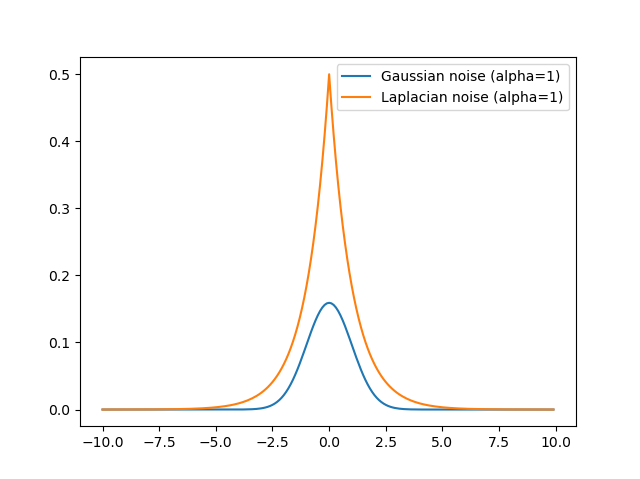
\includegraphics[scale=.4]{C4-1.png}	
	\end{center}
	\title{拉普拉斯分布与高斯分布的对比($\alpha=1$)。}
	\end{figure}
	
	\subsection{Predictive distribution}
	
	\subsection{Equivalent kernel}

\end{document}